\section{Introduction}

% Checked in grammarly
This document is the Software Specification Requirement (SRS) of a website designed to help earthquake victims to acquire the necessary information and give volunteers a chance to donate to help earthquake victims. The website is called \afetbilgi, developed by Middle East Technical University (METU) students and graduates.

\subsection{Purpose of the System}

% Checked in grammarly
\afetbilgi, direct translation to English is `disaster documentation', is an open-source efforted project led by students from METU in Ankara, Turkiye. It aims to provide a clean, verified, and correctly classified information interface for earthquake victims and helpers alike in the aftermath of the tragic earthquake on February 6th, 2023, in Pazarcik, Turkiye. It also offers quick information using confirmed website links, maps, and address tables, along with the relevant contact details of organizations and helpers involved.

\subsection{Scope}

% Checked in grammarly
\afetbilgi\ was established to offer as much information as needed by users in three main categories:
\begin{itemize}
  \item People who are affected by the earthquake (the victims).
  \item Individuals/Organisations who want to help and participate in other government/private efforted procedures in the affected areas.
  \item People from METU who verify and checked any presented links on the websites.
\end{itemize}

The website is primarily responsible for providing tables and datasheets with website links to third-party organizations/contacts details of web places/physical locations which offer/collect help. As indicated here, these links are external and lead out to other websites(outside from \afetbilgi) whose efforts are verified by human resolves (METU students/helpers/site administrators) on the surface-level user experience.

Given how the world is connected with the internet and phones/televised communication, the project developers aim to create a website using these advantageous characteristics via a simple interface in multiple available languages to create fast and easy use of information with no additional and unnecessary obstacles. In areas lacking internet infrastructure that might have been disturbed by the earthquake activities, the website can be distributed via printed-out PDFs, which are shareable via ordinary computers and mobiles, and hand-forwarded physical versions in the forms of leaflets and so on.

Lastly, \afetbilgi\ includes a map functionality if the victim/helper has an internet connection. Any user can locate helper geolocations via terrain/road routes while also being able to quickly view extra details such as written addresses, contact phone details, and previous reviews.

\subsection{System Overview}

This document section will provide detailed information about the system, including all components.

\subsubsection{System Perspective}

% Checked in grammarly
\afetbilgi \cite{afetbilgi} is not part of a more extensive system. It is a standalone and open-source efforted website to verify critical information in the fight against the 6 February 2023 Pazarcik Earthquake and deliver it to disaster victims and those who want to help in an understandable, concise manner in multiple languages.

This information is presented in either the form of legible tables with third-party governmental and private links or an interactable method via a map view interface. If deemed necessary, admin and maintainers can make changes to display newly created or edited data and upload it to the system upon any complaints or suggestions they may get on their contact details.

\begin{figure}[H]
  \centering
  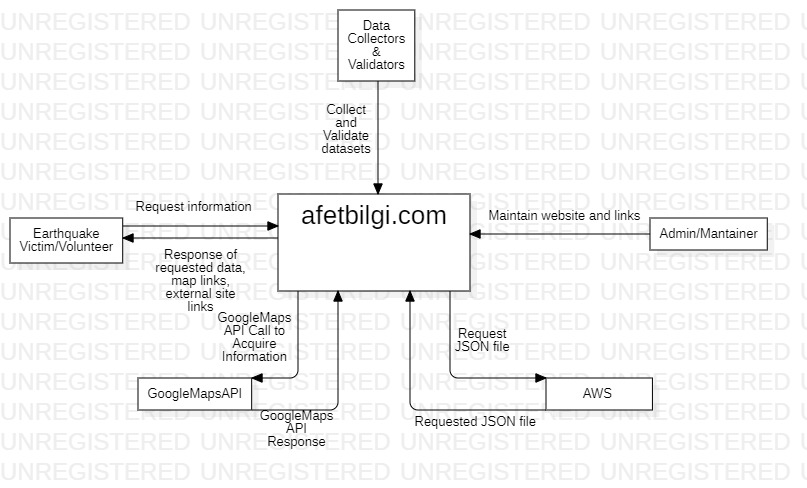
\includegraphics[width=\linewidth]{img/context-diagram.jpg}
  \caption{Context Diagram for \afetbilgi}
\end{figure}

The \afetbilgi\ consists of a combination of small physical and software parts. With the help of interfaces, these parts communicate among themselves and with the user. The following are the interfaces through which interaction occurs:
\begin{itemize}
  \item User interfaces
  \item Software interfaces
  \item Communication interfaces
\end{itemize}
Users interact with the website through their devices connected to the internet, such as cell phones or computers, as the user interface. The software interface enables the website to serve additional features to the user.

\paragraph{User Interfaces}

In order to start using the website, a user should go into the website via a device connected to the internet. The website may have some loading time. After loading, the website is ready for user interactions. Users can interact with \afetbilgi directly to access required information.

The user interface contains \href{https://mui.com/}{MUI} components which are clear buttons and lists. Users can interact with the buttons to access the list of information or access more options related to the chosen information type.

\paragraph{Software Interfaces}

\afetbilgi\ runs mainly JavaScript code with React library. It also uses additional react libraries such as \href{https://mui.com/}{MUI}.

\paragraph{Communication Interfaces}

Since \afetbilgi\ is a website, it communicates via HTTPS (Hypertext Transfer Protocol Secure) and underlying protocols such as TCP/IP. It uses HTTPS to access APIs and servers.

\subsubsection{System Functions}

% Checked in grammarly
\begin{table}[H]
  \centering
  \resizebox{\linewidth}{!}{%
    \begin{tabular}{|p{.3\linewidth}|p{.7\linewidth}|}
      \hline
      \textbf{Function} & \textbf{Summary} \\ \hline
      PDF creation & Users generate PDF versions of the entire website or internal further classified pages per their needs. \\ \hline
      Connect via socials & Victims and helpers can connect with the site administrators and contributors to inform/change anything on the website by clicking on the relevant social app on the main page (discord, etc.). An about section can also be used to contact site administration via formal email methods. \\ \hline
      Search for mobility needs & Lets users click in the relevant section in general needs and bring up information on transportation and evacuation sites. \\ \hline
      Search for necessities & Site user click in the relevant section in general needs and bring up locations as per cities on restaurants, food kitchens, and gas stations. \\ \hline
      Search for housing & Users can click in the relevant section in general needs and bring up dormitories, tenting segmented areas providing shelter. \\ \hline
      Inquire about miscellanous information & In important resources, the website provides a list of resources such as useful articles on efforts and organization contact details. \\ \hline
      Donate and help & People wishing to help the victims are given verified directories of blood banks, charitable private/government organizations for monetary funds, and ongoing digital campaigns to show trends involving support. \\ \hline
      Track hospitals and vets & In the healthcare services section, users can track hospitals, whether for medical supplies, surgical/medicinal help, or even to donate and help in nursing facilities. \\ \hline
      Locate pharmacies & Users can find a directory of pharmacies in the healthcare services if in need of medicinal supplies. \\ \hline
      Language translation & Multiple versions in different languages are provided at the click of a button on any website page. \\ \hline
      Map generation and use & Users can open categorized and labeled locations on interactive maps whether to ask/send help in the affected areas while noting the terrains and routes involved in such areas. The map displays calamity-stricken areas and other areas from other cities taking help as well. \\ \hline
    \end{tabular}
  }
  \caption{System Functions}
\end{table}

\subsubsection{Stakeholder Characteristics}

% Checked in grammarly
There are three main categories of people related to \afetbilgi:
\begin{enumerate}
  \item \textbf{Earthquake victims/ affectees:} These individuals whom the earthquake has directly impacted seek help, support, and information to recover from the disaster. They may be looking for information on how to find shelter, food, medical assistance, and other resources that can help them get back on their feet. The website may provide them with a platform to connect with relief organizations and volunteers and access information on navigating the recovery process.
  \item \textbf{Volunteers:} These individuals want to offer their time, skills, and resources to support the relief and recovery efforts. They may include local volunteers, international volunteers, and disaster response teams. The website may attract volunteers by providing information on how to get involved, where to go, and what support is needed. Their primary use of the website could be to scout places to help from outside the main areas, such as centers transporting essential needs to stricken areas like farther cities such as Ankara and Istanbul. This is the target sector for the Donate or Help category, such as via blood donation, monetary donation, physical volunteer help, etc. Other entities such as relief organizations, government agencies, more prominent sponsors, and potential media outlets can exist within this category.
  \item \textbf{Web developers, Data Collectors, and Site administrators:} These are the website creators responsible for developing, designing, and maintaining the platform. They may include web developers, designers, and other professionals involved in creating and managing the website. These stakeholders may be vested in ensuring the website is accessible, user-friendly, effective, and, most importantly, providing simple, verified information to facilitate relief and recovery efforts without any hurdles.
\end{enumerate}

\subsubsection{Limitations}

% Checked in grammarly
\begin{itemize}
  \item \textbf{Regulatory policies:} Users can access the website without authentication or obstacles. The links themselves to the third party are verified by actual personnel in the site maintainers' team and can be reported by users via given socials and contact us details.
  \item Hardware limitations: Any device such as phones/computers connected to internet infrastructure can access it. In the case of earthquake-stricken infrastructure, PDFs can be generated for website distribution via physical or other electronic means of conveyance.
  \item \textbf{Interface to other applications:} There is no interface to other applications in the in-use build version of the website being serviced to users via the internet, but in the development version(later published after workflow checks), the website is served in the backend with backups of data.
  \item \textbf{Parallel operation:} No parallel operations are involved in this web application, which instead involves different individual directories/maps listing answers to a user's need of information as per his/her selected category/city and language.
  \item \textbf{Audit functions:} There are regularly run Github CI/CD-based workflows that back up site data to the backend cloud at AWS while checking newly added pages/entries for syntax/storage/unreachable DNS link errors.
  \item \textbf{Control functions:} There is no primary control function, but website maintainers / registered contributors are the ones that get to decide what new entries are to be entered/working of existing pages along with viewing reviews or complaints about the website sent to them. The site maintainers also decided on the UI/UX frontend that users interact with in the released website versions and the backend, where the website is hosted/backed up regularly.
  
  \vspace*{\fill}
  \newpage

  \item \textbf{Higher-order language requirements:} Any user who wishes to contribute to the site maintainers should know TypeScript and the React Web framework to work on JSON objects in this static website. Python knowledge assimilates scripts for adding new pages/classes of help/data to the development/published website version.
  \item \textbf{Signal handshake protocols:} For such a static website, it is hosted on the backend and accessed using an IP address (translated from DNS aliases/names categories under afetbilgi.com created by site maintainers) over HTTPS protocol whenever the site domain is typed and entered in any internet browser of choice by the user.
  \item \textbf{Quality requirements:} There is no such limitation in this open-sourced effort that aims to provide fast, reliable information to urgently needed victims and helpers. Hence, the website was published as fast as possible in its initial condition without quality checks during the early earthquake occurrence days, which was also when the website was most used. The only quality procedure involved is a basic shared understanding of the quality of 3rd-party links/external information that the site contributors manually check to get an idea of the reliability of new data before adding it to the site to be accessible by the common public.
  \item \textbf{Criticality of the application:} This website was meant for emergency use and was essential to victims and helpers alike. Hence, it needed at least a basic level of authentication/verification of the links provided, which site contributors did to the best of their abilities, given the minimal time and resources they could receive.
  \item \textbf{Safety and security considerations:} There is no such consideration apart from the fact that site contributors manually check new directories/data to avoid false information, non-renowned/non-existing organizations, fake/fabulous-natured based monetary websites for donations, and so on.
  
  \vspace*{\fill}
  \newpage

  \item \textbf{Physical/Mental considerations:} Multiple languages are provided to be read by any of the widely varying victims/helped involved, along with maps to provide visual prowess in investigating physical routes/terrain/closeness of the locations involved. Pdfs can be generated and shared via physical or electronic means, too, if needed, of the website and its' directories of information listings.
  \item \textbf{Limitations that are sourced from other systems:} There is no such limitation, but Cloudflare is used to provide secure proxy DNS procedures in addition to the website being backed up by a secure AWS bucket instance while employing Vercel in hosting as well. These services are renowned worldwide; hence, given the minimal time of deployment and deliverance, they are the best possible choices for publishing a website.
\end{itemize}

\subsection{Definitions}

\begin{table}[H]
  \centering
  \resizebox{\linewidth}{!}{%
    \begin{tabular}{|p{.3\linewidth}|p{.7\linewidth}|}
      \hline
      \textbf{Term} & \textbf{Definition} \\ \hline
      Python & Computer Programming language to create applications, features, etc. \\ \hline
      React & A JavaScript framework widely used to create websites \\ \hline
      JavaScript & Scripting programming language used to create applets for the internet \\ \hline
      CI/CD & Continuous Integration/Continuous Development \\ \hline
      HTTPS & An internet protocol known as Hyper Text Transfer Protocol Secured \\ \hline
      AWS & Amazon Web Services the provide web hosting servicing \\ \hline
      CloudFlare & A secure DNS hosting service \\ \hline
      Vercel & A web hosting service \\ \hline
      UI/UX & User Interface/User Experience, meant to refer to the frontend part of a web app that the target audience of the website interact with \\ \hline
      PDF & Known as Portable Document Format for easy sharing \\ \hline
      IP & Internet Protocol \\ \hline
      DNS & Domain Name Server \\ \hline
    \end{tabular}
  }
  \caption{Definitions}
\end{table}
